% (C) Marc Lijour, 2017
% This document is licensed under a Creative Commons License BY-SA (feel free to use the code, but all rights are reserved for logos and art)
% https://creativecommons.org/licenses/by-sa/2.5/ca/
% Ayana Consulting presentation template in LaTeX
% This template comes with a first page on a picture background
% Possible improvement in future iterations
% - Test and fix as needed to work on xetex (to use Ubuntu fonts)
% === USAGE===
% Create a file for your LaTeX content (slides, etc), in which you must do the following:
% TODO 1 - set variables defined below
% TODO 2 - include this code by calling: \input{<the name of this document>}
% TODO 3 - Start the document as usual and you're in business; just use \begin{document} and don't forget to conclude with \end{document}
% TODO 4 - Use the custom method \Ayanacoverpage instead of \titlepage to create your cover page
% Voilà!
%
\documentclass[utf8]{beamer}
\usepackage{etoolbox}
%\usepackage[american,french]{babel}
%\usepackage[T1]{fontenc}
%\usepackage[utf8]{inputenc}
% Variables
% ---------------------- USER-DEFINED --------------------------------
\ifdef{\Ayanatitle}{}{\newcommand{\Ayanatitle}{\color{red}Title TBD}}
\ifdef{\Ayanalongtitle}{}{\newcommand{\Ayanalongtitle}{\color{red}Long title TBD}}
\ifdef{\Ayanasubtitle}{}{\newcommand{\Ayanasubtitle}{\color{red}Subtitle TBD}}
\ifdef{\Ayanaauthor}{}{\newcommand{\Ayanaauthor}{\color{red}Author TBD}}
\ifdef{\Ayanadate}{}{\newcommand{\Ayanadate}{\color{red}Date TBD}}
\ifdef{\Ayanasubject}{}{\newcommand{\Ayanasubject}{\color{red}Subject TBD}}
% --------------------------------------------------------------------
\usetheme{Boadilla}
% Set color close to Ayana paletter
%\definecolor{beamer@blendedblue}{RGB}{150,36,36}
\definecolor{beamer@blendedblue}{RGB}{124,42,39}
% Cover Page
\title[\Ayanatitle] {\Ayanalongtitle}
\subtitle{\Ayanasubtitle}
\author{\Ayanaauthor}
\date{\Ayanadate}
\subject{\Ayanasubject}
\usepackage{tikz}
% Try Xetex to use system fonts (pdflatex makes it hard to import a font)
%\usepackage{fontspec}
%\setsansfont{Ubuntu}
%\setmonofont{Ubuntu Mono}

% -- create a custom (command) title page -which has the benefit of not affecting the settings for the rest of the presentation
\newcommand{\Ayanacoverpage}{\frame[plain]{
	\tikz[remember picture,overlay] {
        	\node(bkgd) at ([xshift=0cm,yshift=0cm]current page.center) 
			{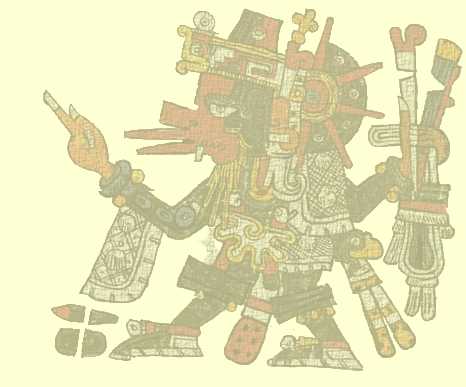
\includegraphics[width=\paperwidth, height=\paperheight]{../../Ayana_Consulting-LaTeX_Templates/images/bkg}};
        	\node(logo) at ([xshift=-4.2cm,yshift=3.5cm]current page.center) 
		 	{
\includegraphics[scale=.06]{../../Ayana_Consulting-LaTeX_Templates/images/logohorizontal-colour}};
        	\node(CC-BY-SA) at ([xshift=5cm,yshift=-4cm]current page.center) 
			{\href{https://creativecommons.org/licenses/by-sa/2.5/ca/}{
\includegraphics[scale=.4]{../../Ayana_Consulting-LaTeX_Templates/images/CC-BY-SA-403x141}}};
	}
	\tikz[remember picture,overlay] {
        	\node(title) at ([xshift=0cm,yshift=0cm]current page.center) 
			%{\Large\color{black}\textbf{{\Ayanalongtitle}}};
			{\Large\color{beamer@blendedblue}\textbf{{\Ayanalongtitle}}};
        	\node(subtitle) at ([xshift=0cm,yshift=-.7cm]current page.center) 
			{\small\color{beamer@blendedblue}\emph{\Ayanasubtitle}};
        	\node(author) at ([xshift=0cm,yshift=-2cm]current page.center) 
			{\small\color{beamer@blendedblue}By~\Ayanaauthor};
        	\node(date) at ([xshift=0cm,yshift=-2.5cm]current page.center) 
			{\tiny\color{beamer@blendedblue}\Ayanadate};
        	\node(footnote) at ([xshift=0cm,yshift=-3.9cm]current page.center) 
			{\TINY\color{beamer@blendedblue}\emph{The Art and Science of Eternal Blossom}};
        	%\node(footnote) at ([xshift=0cm,yshift=-4.1cm]current page.center) 
		%	{\TINY\color{black}\emph{focusing on Blockchain and related technologies}};
    	}
}}
%
% This sets the ColliderX logo at the bottom right corner of each page
\logo{
	
\includegraphics[scale=.07]{../../Ayana_Consulting-LaTeX_Templates/images/Quetzalcoatl_Ourobouros-coloured-same}
}
\AtBeginSection[]
{
  \begin{frame}
    \frametitle{Table of Contents}
    \tableofcontents[currentsection]
  \end{frame}
}
%\usepackage{newunicodechar}
%\usepackage[format=plain,justification=raggedright,singlelinecheck=false]{caption}
\usepackage[format=plain,justification=justified,singlelinecheck=false]{caption}
\usepackage{dirtytalk}
\usepackage{wrapfig}
\usepackage{hyperref}
\usepackage{verbatim}
\usepackage{mathabx}
%\usepackage{MnSymbol}

